\section{Theoretical basics and datasamples}
\label{sec:theorie}

\subsection{The FACT telescope}
FACT (first G-APD Cherenkov Telescope) is the first imaging atmospheric Cherenkov Telescope which uses Geiger-mode avalanche photodiods (G-APD). 
The main purposes of this telescope is being a benchmark for this kind of technology in Cherenkov astronomy.
The second main purpose is to monitor bright and active galactiv nuclei (AGN) in the Terascale.
FACT uses the wobble-mode \ref{fig:wobble} to observe extragalactic sources where the telescope is aimed $\SI{0.6}{\degree}$ next to 
source position in order to estimate the background rate 
in addition to the signal from the source. There is one on-position for the source and 5 off-positions for the background.
The reconstructed events in the on-region are labeled "$N_{on}$" whereas off-region events are labeled "$N_{off}$".
With these parameters, the detector significance is
\begin{equation*}
  \symup{S} = \sqrt{2}\cdot \sqrt{N_{on} \ln\left( \frac{1 + \alpha}{\alpha} \left(  \frac{N_{on}}{N_{on} + N_{off}}\right)\right) +
  N_{off} \ln\left( (1 + \alpha) \left(\frac{N_{off}}{N_{on} + N_{off}}\right)\right)} \, ,
\end{equation*}
where $\alpha$ is ratio of the on-region and off-region. In the wobble-mode with one on-postion and five off positions, the ratio is $\alpha = 0.2$.

\begin{figure}
  \centering
  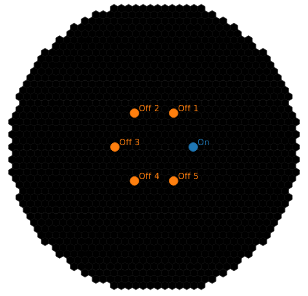
\includegraphics[width=0.8\textwidth]{fact_pics/wobblemode.png}
  \caption{Displayed is the method of the wobble-mode of the FACT detector \cite{ANLEITUNG}.}
  \label{fig:wobble}
\end{figure}

\subsection{Datasamples}
The given datasamples are preprocessed based on the analysis chain typical for data from Cherenkov-Telescopes.
For the shower-events, three attributes of the original particles must be reconstructed: the particle class, the energy and the direction to the origin.
The particle class is typically a gamma-ray or a hadron, for example a proton. The energy is reconstructed via 
regression, most of the time only for gamma-ray candidates. The direction of origin is calculated with a two-dimensional regression in 
either celestial coordinates or detector coordinates.
A typical event is shown in Figure \ref{fig:event}.
\begin{figure}
  \centering
  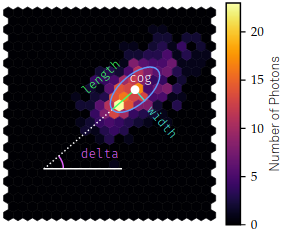
\includegraphics[width=0.6\textwidth]{fact_pics/event.png}
  \caption{Displayed is a typical event with the number of photons stored in each bin. A principal component analysis is additionally displayed to 
  visualize, how the method obtains the parameters \texttt{width} and \texttt{lenth} \cite{ANLEITUNG}.}
  \label{fig:event}
\end{figure}
The standard deviations \texttt{width} and \texttt{length} are calculated from a principal component analysis. 
The middle of the event is called \texttt{cog} and the orientation is defined through angle \texttt{delta} with regards to the x-axis.

To detemine the particle class, the energy and the direction of the origin as well as the detector acceptance, complex simulations are needed to generate 
the training data.
The software \texttt{CORSIKA} was used to generate the airshower, cherenkov-production as well as particle propagation. After that, the software 
saves Cherekov-light detected.
To simulate the FACT telescope, the software \texttt{CERES} was used. Using machine learning techniques, three datasamples were generated:
\begin{itemize}
  \item gammas from point-like source, observed with wobble mode
  \item gammas coming from random directions
  \item protons coming from random directions
\end{itemize}

\subsection{Unfolding}
In physical measurements, the interesting parameters are never measured directly. 
In the astrophysics department energy deposits are used to yield the original attributes of the particles. This is called an "inverse problem" and can be described by 
the equation
\begin{equation}
  g(y) = \int A(y,x) f(x) \symup{d}x + b(y) \, ,
  \label{eqn:convo}
\end{equation}
where f(x) is the probability density function of interest, depending on the physical parameter x. 
The function g(y) is the probability density function of the measured parameter y and b(y) is the background. A(y,x) is the concolution core represented by the detector.
To solve this problem, unfolding techniques are used. \par 
In a discrete form, equation \eqref{eqn:convo} can be written as
\begin{equation}
  \symbf{g} = \symbf{A}\symbf{f} + \symbf{b} \, .
\end{equation}
Here, $\symbf{g}$ is the histogram of the estimated gamma-energies and $\symbf{f}$ is the histogram of the true gamma-energies.
$\symbf{A}$ is the migration matrix constructed from the estimated and true gamma energies and $\symbf{b}$ is the background derived from the off-regions.

\subsubsection{Naive SVD unfolding}
An easy method to invert equation \eqref{eqn:convo}, is to invert the 
matrix $A$. In the case of non-quadratic matrices, the 
Moore-Penrose-Pseudoinverse needs to be calculated using
\begin{equation}
  \hat{\symbf{f}} = \symbf{A}^{+}(\symbf{g} - \symbf{b}) \, .
  \label{eqn:svd}
\end{equation}
This solution is equivalent to the method of least squares.

\subsubsection{Poisson-likelihood-unfolding}
If $\symbf{g}$ follows a poisson distribution, a maximum-likelihood fit can be performed.
The probability to measure $g_i$ is
\begin{align}
  \symup{P}(g_i) &= \mathcal{P}(g_i, \lambda_i) \\
  \shortintertext{with}
  \symbf{\lambda} &= \symbf{A}\symbf{f} + \symbf{b} \\
  \intertext{minimizing the negative log-likelihood yields}
  -\ln(\mathcal{L}) &= \sum_{i=1}^{M} = -g_i \ln(\lambda_i) + \lambda_i \\
  \intertext{the estimator for $\symbf{f}$ is then}
  \hat{\symbf{f}} &= \text{argmin}(-\ln(\mathcal{L}(\symbf{f}|\symbf{A},\symbf{g},\symbf{b})))\, .
\end{align} 
